
\chapter{基于深度学习的骨髓血细胞检测算法设计与实现}
\section{引言}
骨髓血细胞形态学检查是血液疾病诊断的重要依据,主要通过人工镜检来完成,上述过程繁琐枯燥,可靠性差。
在骨髓血细胞自动化识别算法中,骨髓血细胞检测是将血细胞从涂片图像中定位并裁剪得到单一的血细胞图像,该过程是后续分类识别基础,
直接影响血液疾病诊断的结果,因此一直都是医学图像处理的热点研究方向之一。
目前基于深度学习的目标检测算法在很多领域都有广泛应用,如自动驾驶、安防监控、人脸识别、医学影像诊断等,其目的是定位或者跟踪相关目标。

根据文献调研,目前血细胞检测主要是对血细胞图像中的红细胞、白细胞与血小板进行检测。
检测算法主要基于通用的深度学习目标检测算法,包括了单阶段检测算法与两阶段检测算法。
在两阶段方法中,通过区域举荐网络生成少量感兴趣区域,并将这些区域提取到的特征输入到后续的分类与回归分支中。
在单阶段算法中,如SSD、YOLO等网络直接将全部图像作为输入,学习类别概率与边界框位置。
两类方法各有优劣,本章对这些方法进行阐述,并进行性能分析,最终选取性能较好的RetinaNet作为骨髓血细胞检测的基线模型。


\section{双阶段目标检测网络}
\label{section:faster-rcnn}
快速区域卷积网络(Faster-RCNN)是目标检测领域最为经典的双阶段检测器,其网络架构如图\ref{fig:faster_rcnn}所示,主要由
骨干网络特征提取器(BackBone)、区域举荐网络(Region proposal Network,RPN)与分类回归网络(R-CNN)这三部分组成。骨干网络为深度卷积神经网络,
用于图像特征提取。RPN网络在提取的特征图上快速生成区域坐标与相应前景分数,这些区域用于后续的分类与坐标回归。
R-CNN网络对于这些区域首先进行ROI池化(Region of Interest Pooling)将区域转换为特定大小的特征图,然后这些特征图会分别进入到
分类分支与回归分支,得到待检测目标的类别与位置信息。

\begin{figure}[htbp]  
   \centering   
   \includegraphics[width=0.9\linewidth]{faster_rcnn.jpg}   
   \caption{快速区域卷积神经网络结构示意图}   
   \label{fig:faster_rcnn} 
\end{figure}  

\subsection{骨干网络}
骨干网络是深度卷积神经网络的主体部分,用于提取图像抽象的语义特征,为后续任务提供图像的嵌入特征向量表示。
因此,骨干网络的性能对于整体网络性能具有很大的影响。常用的骨干网络有VGG、ResNet、DenseNet与Inception等,
其中ResNet是应用最为广泛的骨干网络,其特点是引入了残差模块,可以实现很深层的卷积网络。

综合考虑模型的精度、速度、参数量等因素,本节模型选择的骨干网络均为ResNet50,其结构如图~\ref{fig:resnet50}所示。
ResNet50总共由五个阶段(stage)构成,第一个阶段由一个$7\times7$的卷积组成,可视作对图像的预处理。
其余阶段均是由沙漏模块(BottleNeck)堆叠而成,第二到第五阶段分别有3、4、6、3个沙漏模块。若输入图像的大小为$224\times224\times3$
每经过一个stage,特征图的大小减小为原来的一半,通道数变为原来的两倍。五个阶段输出的特征图分别为$C_1, C_2, \dots, C_5$,
其中$C_5$特征图的大小为$7\times7\times2048$。最后特征图经过均值池化变为2048的向量,经过全连接层用于分类识别。

\begin{figure}[htbp]      
  \centering       
  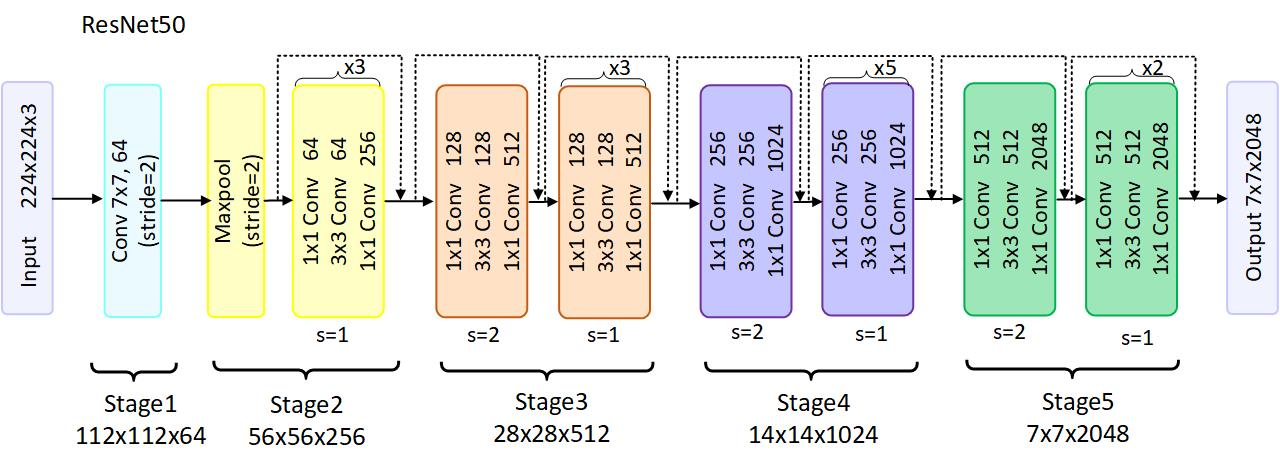
\includegraphics[width=0.9\linewidth]{resnet50.jpg}       
  \caption{ResNet50网络结构示意图}       
  \label{fig:resnet50}  
\end{figure}   

沙漏(BottleNeck)模块结构如图\ref{fig:bottleneck}所示,该网络第一个卷积层使用$1\times1$的卷积核来减少通道数量。
第二个卷积层的卷积核大小为$3\times3$,当stride为1时,特征图大小不变,stride=2时,特征图大小变为原来的一半。第三个卷积层采用$1\times1$卷积
恢复特征图的通道数。由于中间层的维度较小类似于沙漏,因此称为沙漏结构。该结构可以有效降低网络的参数量与计算量。
该结构还包括了一个残差模块,通过一个$1\times1$的卷积确保输入与输出的通道数相同后,在与输出直连相加。残差连接可以让网络更好的学习高层特征,
同时避免网络浅层部分梯度消失或爆炸等问题。图中BN为批归一化层、ReLU为激活函数。

\begin{figure}[htbp]        
  \centering          
  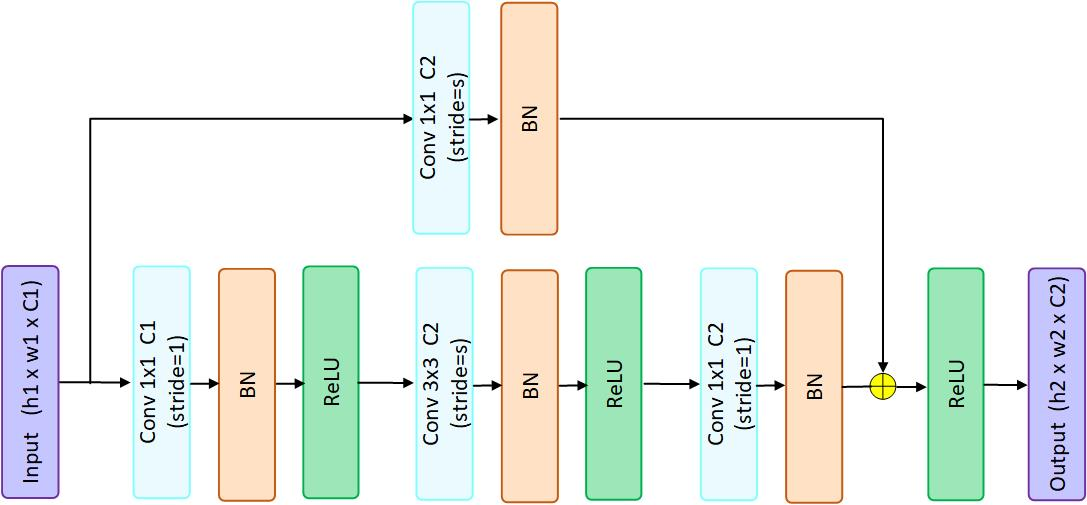
\includegraphics[width=0.7\linewidth]{bottleneck.jpg}          
  \caption{BottleNeck模块结构示意图}          
  \label{fig:bottleneck}   
\end{figure}    

\subsection{特征金字塔网络}

特征金字塔网络(Feature Pyramid Network,FPN)主要用来解决多尺度的目标检测问题。骨干网络特征提取器输出不同尺度的特征图,这些特征图的感受野不同。
高层特征图感受野比较大,用来检测大尺寸目标,浅层的特征图感受野较小,用来检测小尺寸目标。
但是浅层特征图的表达能力较弱,通常只有纹理、边缘形状、明暗等细节信息,而高层特征图则包含更加丰富的全局信息。
为解决浅层网络特征表达能力有限的问题,Lin等\cite{2017Feature}引入了特征金字塔网络。该网络将顶层特征逐级向下传递并与浅层特征融合,
使得浅层特征可以同时兼顾细节与整体具有更加丰富的特征表达。ResNet50骨干网络构建特征金字塔的结构如图~\ref{fig:fpn}所示。
图中$C_1,C_2 \cdots C_5$为ResNet骨干网络生成的不同尺度特征图,相邻两个阶段的特征图在尺寸上为二倍缩放的关系。
自顶向下的融合过程经过上采样与通道调整使得特征图的尺寸一致后再相加融合。以$P_4$特征图的生成为例,$P_5$由$C_5$特征图经过$1\times1$、通道数为256的卷积层得到。
$P_5$经过二倍上采样(由反卷积实现)与$C_4$经过$1\times1$、通道数为256的卷积的结果相加得到$P_4$。其他特征图同样由上述过程生成。
最后FPN使用$3 \times 3$卷积对融合后的特征图进行平滑处理消除直接相加可能导致的融合不充分问题。至此,完成了特征金字塔的构建。

\begin{figure}[htbp]            
  \centering             
  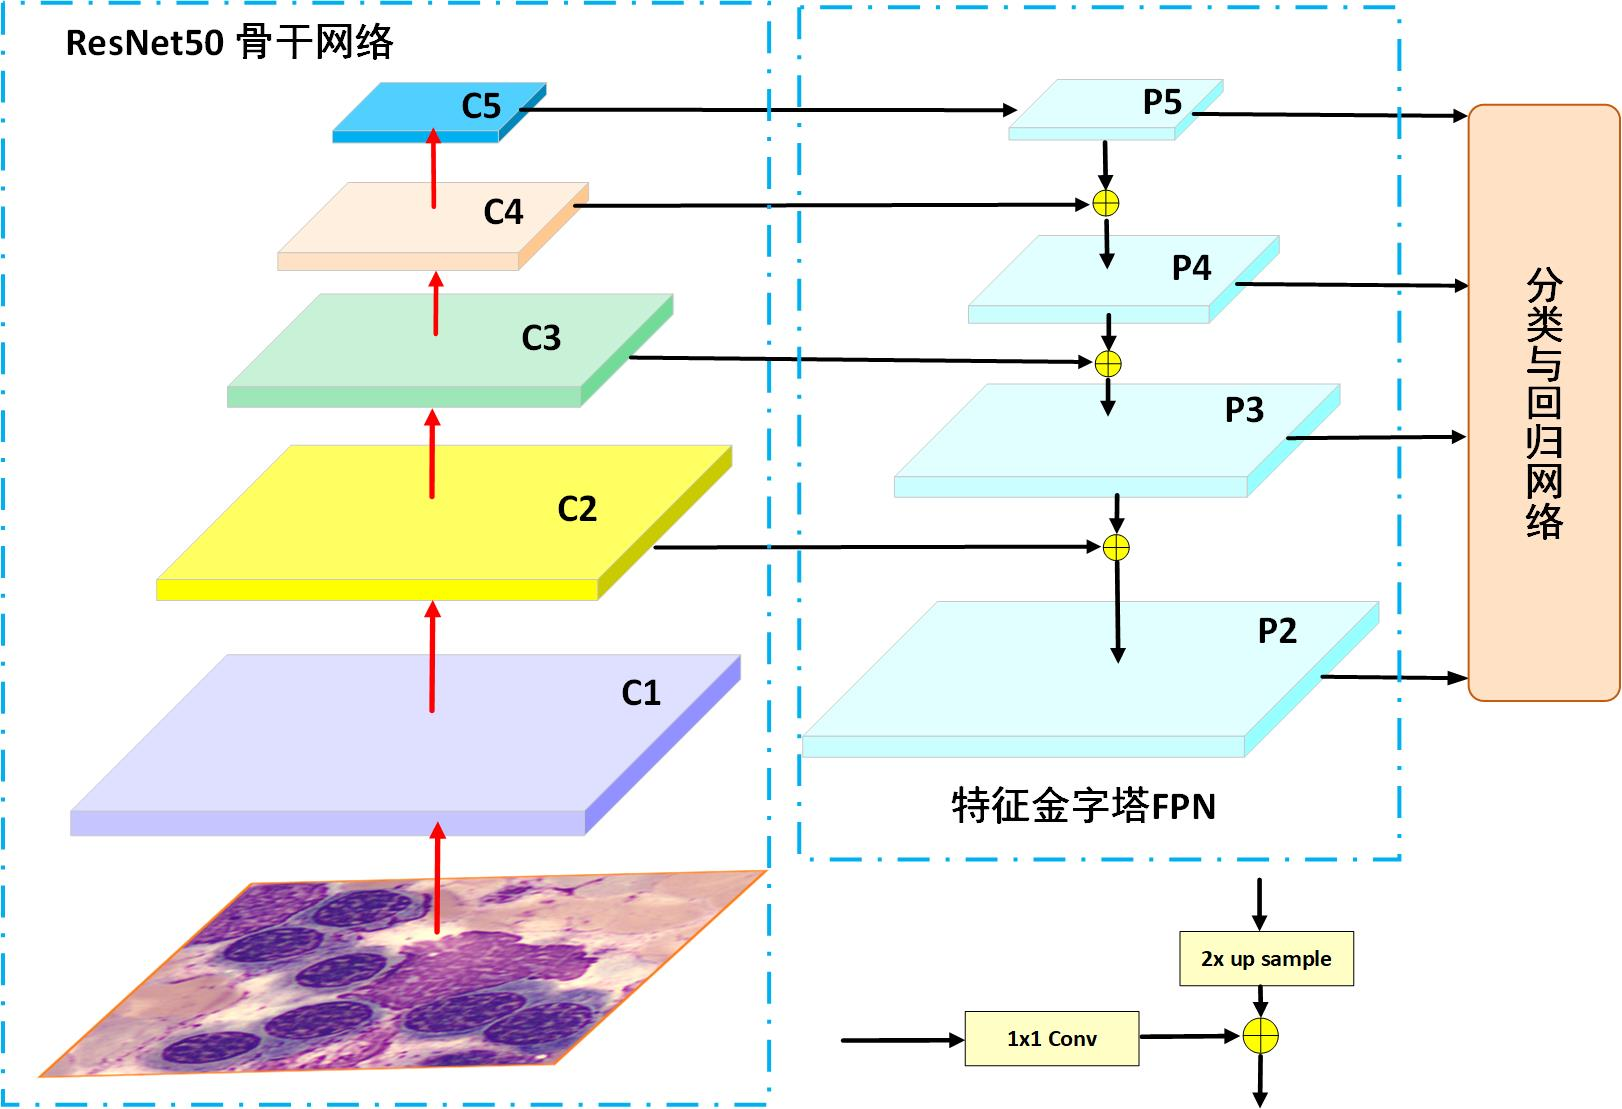
\includegraphics[width=0.65\linewidth]{fpn.jpg}             
  \caption{特征金字塔网络结构示意图}             
  \label{fig:fpn}    
\end{figure}    

\subsection{区域举荐网络}

区举荐网络(Region Proposal Network, RPN)基于骨干网络提取的特征图生成一系列候选框区域,用于后续分类识别。
RPN网络结构如图~\ref{fig:rpn}所示,包含了两个分支,上面一条分支用于预测每个锚框属于前景的分数。
下面一条分支用于计算锚框边界坐标的回归信息,以生成更加精准的区域坐标。最后生成的候选框区域综合了前景分数与坐标修正,
实现了目标的初步定位。

\begin{figure}[htbp]              
  \centering                
  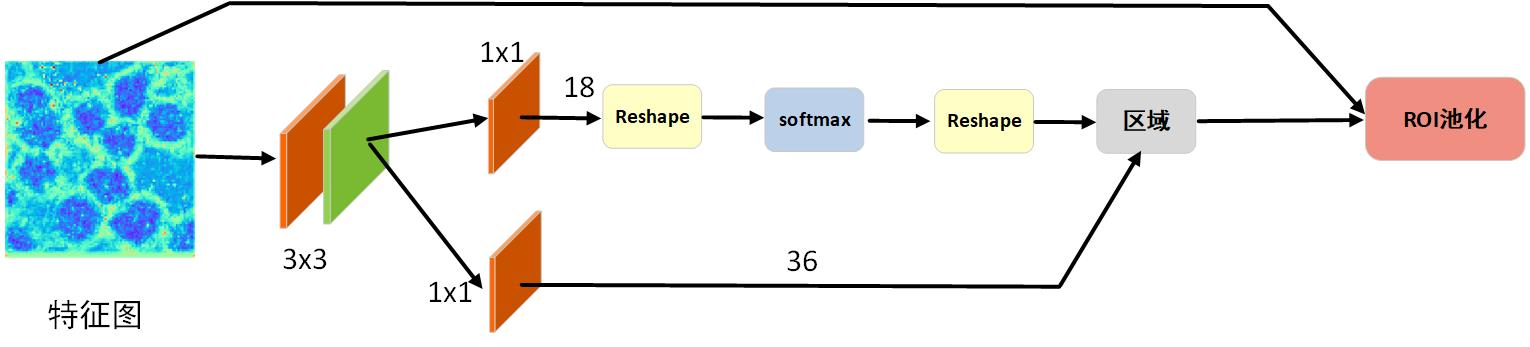
\includegraphics[width=0.90\linewidth]{rpn.jpg}                
  \caption{特征金字塔网络结构示意图}                
  \label{fig:rpn}     
\end{figure}   

锚框是RPN网络根据预先定义的参数生成的一些列矩形区域,对于特征图上的每个锚点会生成$k$个锚框,通常将$k$设置为$9$。如图\ref{fig:anchor}(a)所示,
九个锚框有三种尺寸与三种长宽比,锚框尺寸由数据集目标先验信息与特征图大小决定,
尺度变化范围为$2^0, 2^{\frac{1}{3}},  2^{\frac{2}{3}}$,长宽比通常设定为$0.5, 1, 2$。以骨髓血细胞图像为例,原图尺寸为
$363 \times 360 \times 3$,首先经过缩放与填充转大小换为$832 \times 800 \times 3$,所有anchor的尺寸在$32 \times 32$ \textasciitilde
$812 \times 812$,几乎可以覆盖各个尺寸的目标。以$P_2$特征图为例,该特征图的尺寸为$208 \times 200$,缩放尺度为4,九种anchor的尺寸分别为
$23 \times 45,\quad32 \times 32,\quad45 \times 23,\quad29 \times 57,\quad40 \times 40,\quad57 \times 29,\quad36 \times 72,\quad51 \times 51,\quad72 \times 36$。

\begin{figure}[htbp]
	\centering
	\begin{subfigure}{0.45\linewidth}
		\centering
		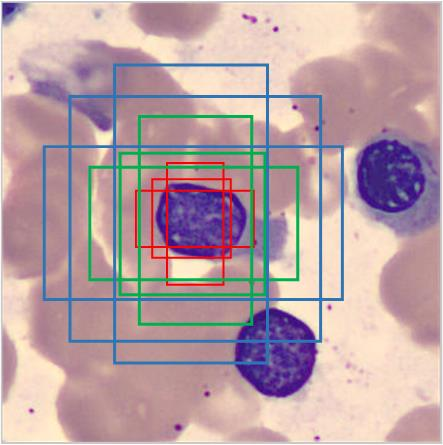
\includegraphics[width=0.95\linewidth, height=0.95\linewidth]{anchor_a.jpg}
    \caption{}
	\end{subfigure}
	\centering
	\begin{subfigure}{0.45\linewidth}
		\centering
		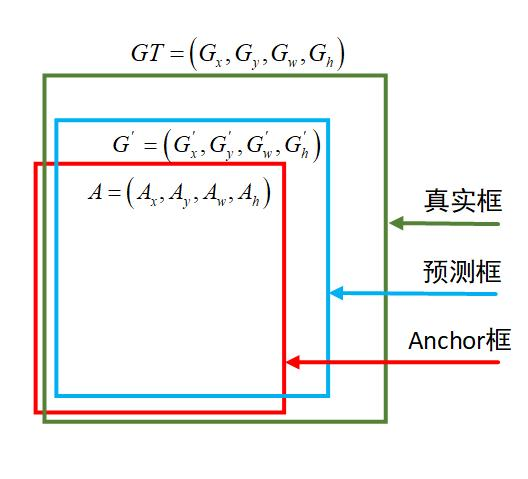
\includegraphics[width=0.95\linewidth, height=0.95\linewidth]{anchor_b.jpg}
    \caption{}
	\end{subfigure}
	\caption{(a) Anchor在图像中的示意图, (b) Anchor、预测框与真值框之间的关系}
	\label{fig:anchor}
\end{figure}

特征图经过预测前景分支后输出的尺寸为$h\times w \times 2k$,
对应锚点的$k$个锚框,每个锚框有前景与背景两种分数。经过坐标回归分支后得到尺寸为$h\times w \times 4k$的
坐标回归结果。我们采用$(x, y, w, h)$这样的四维向量来表示矩形框,分别代表矩形框的中心与宽高。
如图\ref{fig:anchor}(b)所示, 红色框A为按照预先定义生成的锚框$A = \left( {{A_x},{A_y},{A_w},{A_h}} \right)$,
绿色框代表目标的真值框$GT = \left( {{G_x},{G_y},{G_w},{G_h}} \right)$。坐标回归分支希望学习到一个映射
$F\left(A_{x}, A_{y}, A_{w}, A_{h}\right)=\left(G_{x}^{\prime}, G_{y}^{\prime}, G_{w}^{\prime}, G_{h}^{\prime}\right)$,
使得原始的锚框A经过映射后得到的预测框$G^{\prime}$能够更加接近真实框$GT$。

变换$F$中包含的参数通过坐标回归分支得到$d_{*}(A)=W_{*}^{T} \cdot \phi(A)$,其中$\phi(A)$为锚点对应的特征向量,
$W_{*}$为$1\times1$卷积层需学习的参数,$d_{*}(A)=d_{x}(A), d_{y}(A), d_{w}(A), d_{h}(A)$,锚框A与预测框$G^{\prime}$
的坐标关系如式~\ref{eq:bbox_reg1}所示。
\begin{equation}
  \begin{array}{cc}
    G_{x}^{\prime} =A_{w} \cdot d_{x}(A)+A_{x} & G_{y}^{\prime} = A_{h} \cdot d_{y}(A)+A_{y} \\
    G_{w}^{\prime} =A_{w} \cdot \exp \left(d_{w}(A)\right) & G_{h}^{\prime} =A_{h} \cdot \exp \left(d_{h}(A)\right)
  \end{array}
  \label{eq:bbox_reg1}
\end{equation}

真实框GT与锚框A之间的平移量$(t_{x}, t_{y})$与尺度因子$(t_{w}, t_{h})$的变换计算如式~\ref{eq:bbox_reg2}所示。
\begin{equation}
  \begin{array}{cc}
    t_{x}=\left(G_{x}-+A_{x}\right) / A_{w} & t_{y}=\left(G_{y}-A_{y}\right) / A_{h} \\
    t_{w}=\log \left(G_{w} / A_{w}\right) & t_{h}=\log \left(G_{h} / A_{h}\right)
  \end{array}
  \label{eq:bbox_reg2}
\end{equation}

坐标回归分支网络在训练时的优化目标是让预测值$d_{*}(A)$与真实变换系数$t_{*}$之间的差距最小,选择smooth-L1损失函数进行优化。
在测试时,网络输出修正的坐标变换信息将锚框修正,用于后续处理。
\begin{equation}
  {\hat W_*} = {{\mathop{\rm argmin}\nolimits} _{{W_*}}}\sum\limits_i^n {{{{\mathop{\rm smooth}\nolimits} }_{{L_1}}}
  \left( {t_*^i - W_*^T \cdot \phi ({A^i})} \right)}  + \lambda \left\| {{W_*}} \right\|
  \label{eq:bbox_reg3}
\end{equation}
\begin{equation}
  \operatorname{smooth}_{L_{1}}(x)
  =\left\{\begin{array}{rr} 0.5 x^{2} & \text { if }|x|<1 \\ |x|-0.5 & \text { otherswise, } \end{array}\right.
  \label{eq:bbox_reg4}
\end{equation}

\subsection{分类与回归网络}
RPN网络生成的候选区域大小形状各不相同,需要经过ROI池化保证尺寸相同。首先将候选区域对应位置映射到特征图上,将对应特征图区域
划分为$pool_w \times pool_h$的网格,在每个网格区域内进行最大池化,这样每个区域转化为$pool_w \times pool_h$固定大小输出。

\begin{figure}[htbp]                  
  \centering                   
  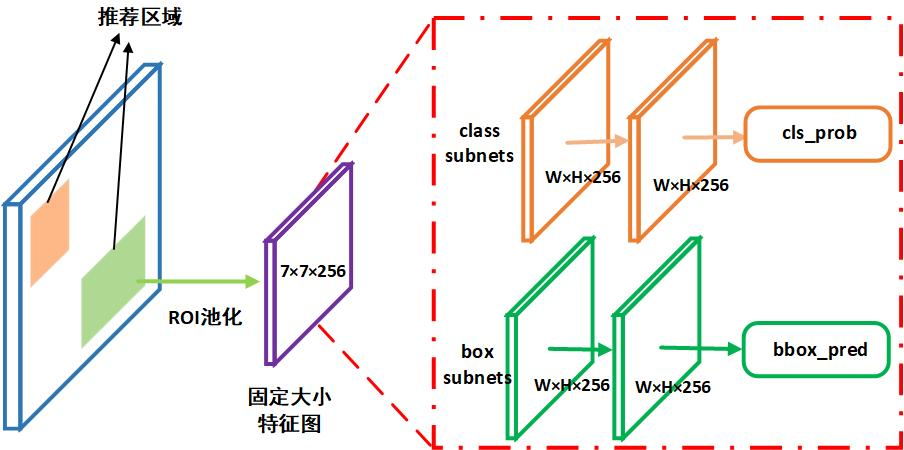
\includegraphics[width=0.75\linewidth]{subnets.jpg}                   
  \caption{分类与回归网络结构示意图}                   
  \label{fig:subnets}      
\end{figure}   

分类网络使用ROI池化后的特征图,经过全连接层与Softmax函数输出分类概率向量,在训练时使用交叉熵损失函数进行优化。
回归分支与RPN网络部分的坐标回归分支类似,目的是为了获得更加精确的检测框坐标。

\section{单阶段目标检测网络}

\subsection{网络结构}
单阶段检测器如SSD、RetianNet、YOLO系列等具有较快的检测速度与较高的检测精度,通常用于实时目标检测。
单阶段检测器在特征图上进行密集检测,对所有的锚框均进行分类与回归。
在图像中大量的锚框都属于负样本,因此单阶段检测器在训练阶段面临着严重的正负样本不均衡问题,大量易分的负样本
主导了损失函数的训练,使得网络难以对正样本进行学习,影响参数收敛,网络性能差。
两阶段网络如Faster-RCNN通过区域举荐网络对所有锚框进行前景分数预测,并将可能包含目标的少量候选框传给后续的分类回归网络进行识别,
有效的控制了正负样本比例,很好的解决了上述问题。

为解决单阶段检测器中极度不平衡的正负样本问题,Lin~\cite{lin2017focal}等提出了一种简单且实用的焦点损失函数(Focal Loss),并设计了RetianNet网络。
在该损失函数引导下,网络增加了对难以区分正样本的关注,减少了对易分辨背景样本的关注。RetinaNet网络结构如图~\ref{fig:retinanet}所示,由骨干网络、特征金字塔网络与分类回归网络组成,
网络主体结构在~\ref{section:faster-rcnn}节已进行详细阐述。

\begin{figure}[htbp]                     
  \centering                      
  \includegraphics[width=0.80\linewidth]{retinanet.jpg}                      
  \caption{分类与回归网络结构示意图}                      
  \label{fig:retinanet}       
\end{figure}   

\subsection{焦点损失函数}
焦点损失是基于交叉损失函数提出,在深度学习中,交叉熵用来衡量模型预测结果分布与真实结果分布之间的差异性,一般用于分类任务。
假设有$N$个样本,类别数为$C$,$y_{ij}$表示第$i$个样本属于第$j$类的标签,取值为$0, 1$。$\hat{y_{ij}}$表示模型预测第$i$个样本属于第$j$
的概率,则交叉熵损失函数如式~\ref{eq:ce_loss}所示:
\begin{equation}   
  {\rm{CE}}\_{\rm{Loss}}(y,\hat y) =  - \frac{1}{N}\sum\limits_{i = 1}^N {\sum\limits_{j = 1}^C {{y_{ij}}} } \log \left( {\widehat {{y_{ij}}}} \right)
  \label{eq:ce_loss} 
\end{equation}

在二分类问题中,只有两个正负样本,若$p$表示预测为正样本的概率,$1-p$表示预测为负样本的概率,样本标签取值为$0,1$,则二元交叉熵如式所~\ref{eq:bce_loss}示:
\begin{equation}         
  \operatorname{BCE}=\left\{\begin{array}{ccc} -\log (p), & \text { if } & y=1 \\ -\log (1-p), & \text { if } & y=0 \end{array}\right.  
  \label{eq:bce_loss}   
\end{equation} 

常见解决正负样本不平衡的方法是引入$\alpha$参数平衡正负样本损失函数的权重。该参数由正负样本比例决定$\frac{\alpha}{1-\alpha} = \frac{n}{m}$,式中$n$为负样本数量,
$m$为正样本数量。
\begin{equation}            
  \operatorname{BCE}=\left\{\begin{array}{ccc} -\alpha \log (p), & \text { if } & y=1 \\ -(1-\alpha) \log (1-p), & \text { if } & y=0 \end{array}\right.    
  \label{eq:bce_loss_alpha}    
\end{equation} 

焦点损失在平衡二元交叉熵损失基础上加入了难易调整因子$\gamma$,训练过程中,大量的锚框都属于易分的背景样本,这些置信度较高的样本
对于模型效果提升影响较小。焦点损失对于高置信度样本进行惩罚,降低其损失函数中的权重$(1-p_t)^{\gamma}$,使得网络关注到难分的正负样本。
焦点损失如式~\ref{eq:focal_loss}所示。$\gamma=0$时焦点损失等价于平衡二元交叉熵损失函数,$\gamma=2$时网络的效果较好,当分类概率$p_t$为0.9时,其损失函数权重降低100倍。
而分类概率$p_t = 0.5$时,损失函数权重仅降低四倍。这使得网络在训练时能不断地聚焦在那些学习较差的样本上,梯度更新方法主要困难样本决定。$\alpha$是类别权重,正负样本的$\alpha$通常设置为
$(0.25, 0.75)$。
\begin{equation}               
  \begin{array}{*{20}{c}} {{\rm{Focal\_Loss}}\left( {{p_t}} \right) =  - \alpha {{\left( {1 - {p_t}} \right)}^\gamma }\log \left( {{p_t}} \right)}\\ 
    {{p_t} = \left\{ {\begin{array}{*{20}{c}} {p,}&{{\rm{ if }}}&{y = 1}\\ {1 - p,}&{{\rm{ if }}}&{y = 0} \end{array}} \right.} \end{array}    
  \label{eq:focal_loss}     
\end{equation} 

\subsection{网络预测}

在网络的预测推理阶段,RetinaNet在特征金字塔输出的多尺度特征图上进行预测。对于骨髓血细胞图像首先通过双线性插值缩放到$832 \times 800$大小,
其特征图$P_2, P_3 \cdots, P_5$的大小分别为$208 \times 200$、$104 \times 100$、$52 \times 50$、$ 26 \times 25$、$13 * 13$,特征图上的每个锚点
输出9个锚框,对于一张骨髓血细胞图像,网络总共输出$55250 \times 9$个检测结果。每个检测结果包括了一个分类置信度向量与一个四维坐标回归向量,
根据坐标回归向量可以计算出检测框在原始图像上的坐标。对于每个骨髓血细胞类别,大量的检测框均为背景区域,首先将置信度低于0.05的检测框滤除。
然后对检测框按照置信度从高到低进行排序,选取前1000个检测框进行非极大值抑制(Non-Maximum Suppresion,NMS)去除重复的检测框。NMS的过程如下:
首先从置信度最高的框开始,计算它与剩余框的交并比(IOU),并去除交并比大于阈值(通常为0.5)的框。然后在剩余框中继续选择置信度最高的框重复上述过程,
最后保留的框为非极大值抑制后处理后的结果。最终合并所有血细胞类别的检测结果,选择置信度最大的前100个框作为当前图片的检测框结果。


\section{算法实现与实验结果分析}

研究初期,我们需要对比不同目标检测网络的性能,确定骨髓血细胞检测的基线模型,然后在此基础上进行改进。
在双阶段网络中,我们选择了Faster-RCNN、Cascade-RCNN网络,在单阶段网络中,我们选择RetinaNet与YOLOV3。
上述网络都是经典的具有代表性的检测网络。我们比较了不同网络的参数量与浮点计算量与在骨髓血细胞数据集上的检测精度。
此外,我们探索了网络在仅做检测与检测识别一体化任务上性能的差异。

\subsection{实验环境}

\subsubsection{数据集介绍}
\label{section:dataset}

骨髓血细胞图像来自邃蓝智能科技(上海)有限公司合作医院提供,首先采用第2.1小节阐述的主动学习标注策略进行边界框的标注。
我们总共标记了6821张血细胞图像,训练集与测试集按照4:1的比例进行随机划分,训练集包含了5456张图像,测试集包含了1365张图像。
通常每个图像中包含1到10个有核血细胞,数据集总共标记了11352个血细胞,训练集有9065个血细胞,测试集有2287个血细胞。数据集的分布如
表~\ref{table:cell_detect}所示:

\begin{table}
  \caption{骨髓血细胞检测数据集分布}   
  \centering 
  \label{table:cell_detect}
  \begin{tabular}{ccccc}
    \toprule[2pt]
    序号 & 类别名  &  类别简写 & 训练集数量 & 测试集数量 \\
    \midrule[1.5pt] 
    1 & 原始细胞 & Prim & 1856 & 467 \\ 
    2 & 淋巴细胞 & Lym & 996 & 226   \\ 
    3 & 单核细胞 & Mono & 206 & 52   \\ 
    4 & 浆细胞 & Plas & 272 & 70   \\ 
    5 & 红细胞 & Red & 1880 & 503   \\ 
    6 & 早幼粒细胞 & Promy & 357 & 107   \\ 
    7 & 嗜中性中幼粒细胞 & Myelo & 701 & 150   \\ 
    8 & 嗜中性晚幼粒细胞 & Late & 503 & 144   \\ 
    9 & 嗜中性杆状核细胞 & Rods & 998 & 241   \\  
    10 & 嗜中分叶核细胞 & Lobu & 821 & 195   \\  
    11 & 嗜酸性粒细胞 & Eosl & 475 & 132   \\  
    \hline
    总计 &   &   & 9065 & 2287 \\
    \bottomrule[2pt]      
  \end{tabular} 
\end{table}

\subsubsection{评价指标}

在目标检测领域,通常使用检测框与真实框的交并比(IOU)来判断检测框是属于正样本还是负样本。交并比的定义如图~\ref{fig:iou}所示,对于预测框A与真实框B,
IOU值等于两个矩形框的交集面积$S(A \cap B)$与并集面积$S(A \cup B)$的比值。IOU的取值范围为$0 \sim 1$,值越大表示两个矩形相似程度越高。
\begin{figure}[htbp]                     
  \centering                      
  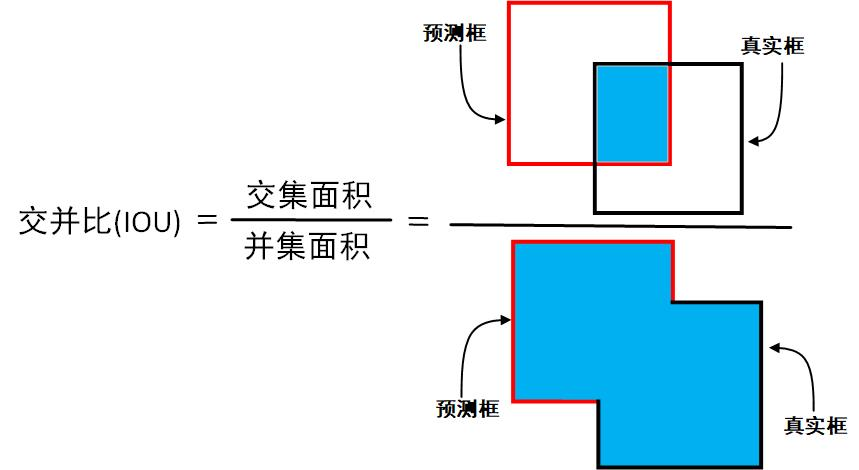
\includegraphics[width=0.60\linewidth]{iou.jpg}                      
  \caption{IOU计算示意图}                      
  \label{fig:iou}       
\end{figure}   

在深度学习中,TP(True Positive)表示被正确检测为正类的正样本;FP(False Positive)表示被错误检测为正类的负样本;
TN(True Negative)表示被正确检测为负类的负样本。FN(False Negative)表示被错误检测为负类的正样本。
对于检测任务,需要根据检测框的置信度分数与交并比来判断
以图~\ref{fig:confusion}为例,绿色框为真实框,红色框为网络检出框。
第一张图中检测框与真实框IOU大于阈值,且类别正确,为真正例TP。第二张图中IOU大于阈值,但是类别检测错误,分叶核(Lobu)真实类别被错误检测为杆状核(Rods)类别(FP)。
第三张图中,检测框与所有真实框IOU均小于阈值,背景类被错误检测为Lobu类(FP)。第四张图片未检出,Lobu类别被错误检测为背景类(FN)。

\begin{figure}[htbp]
	\centering
  \begin{subfigure}{0.24\linewidth}
    \centering
    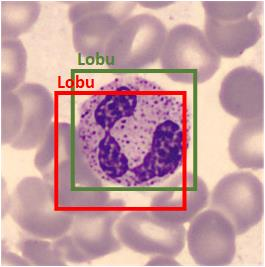
\includegraphics[width=0.95\linewidth, height=0.95\linewidth]{det1.jpg}
    \caption{检测正确TP}
  \end{subfigure}
	\centering
	\begin{subfigure}{0.24\linewidth}
		\centering
		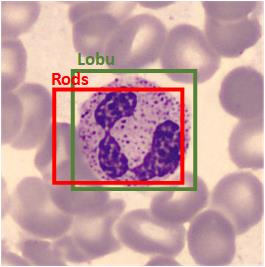
\includegraphics[width=0.95\linewidth, height=0.95\linewidth]{det2.jpg}
    \caption{分类错误FP}
	\end{subfigure}
	\centering
	\begin{subfigure}{0.24\linewidth}
		\centering
		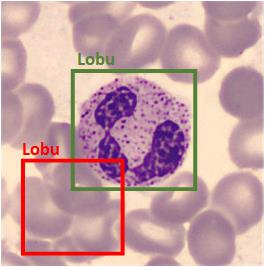
\includegraphics[width=0.95\linewidth, height=0.95\linewidth]{det3.jpg}
    \caption{IOU小于阈值BG}
	\end{subfigure}
	\centering
	\begin{subfigure}{0.24\linewidth}
		\centering
		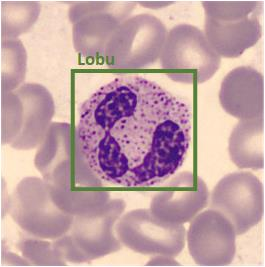
\includegraphics[width=0.95\linewidth, height=0.95\linewidth]{det4.jpg}
    \caption{未检出FN}
	\end{subfigure}
	\caption{检测类型判别}
	\label{fig:confusion}
\end{figure}

目标检测常用的评价指标有精准率(precision)、召回率(recall)、PR曲线、平均精度(Average Precision,AP)与平均精度均值(Mean Average Precision,mAP)。

精准率是指预测正确的正样本数量与所有预测为正样本数量的比值,如式~\ref{eq:precision}所示:
\begin{equation}               
  Precision = \frac{TP}{TP + FP}
  \label{eq:precision}     
\end{equation} 

召回率是指预测正确正样本数量与所有正样本数量的比值,如式~\ref{eq:recall}所示
\begin{equation}               
  Precision = \frac{TP}{TP + FN}
  \label{eq:recall}     
\end{equation} 

PR曲线是以召回率为横坐标,以精确率为纵坐标绘制的曲线。在绘制某一类别PR曲线时,将检测框按照置信度从高到低
进行排序,设定多组置信度阈值,根据交并比会得到多组精确率与召回率,最后将这些点连接起来得到最终的PR曲线。
随着召回率的提高,检测的精确率会降低,曲线越靠近右上角代表网络的检测性能越好
平均精度是PR曲线下的面积,即在多组召回率下的平均检测精确率。AP值越大代表模型的性能越好。
平均精度均值(mAP)是对所有类别的平均精度求均值,通常用来衡量网络的检测效果。

\subsubsection{实验设置}
我们在Linux操作系统下的NVIDIA TITAN V显卡上训练模型。训练使用的深度学习框架为Pytorch1.13.1,批量大小设置为16。
优化器使用随机梯度下降算法(SGD),动量设置为0.9,权重衰减设置为5e-4。学习率初始化为0.001,网络总共训练36个轮次,
在第16与第28个轮次,学习率变为原来的$1/10$。RetianNet中Focal Loss中正负样本平衡参数$\alpha=0.25$,难易调整参数$\gamma=2$。
数据集原始图像大小为$363 \times 300$,为了更好的检测小目标,图像经过双线性插值与填充扩大到$832 \times 800$。
我们基于迁移学习的方式进行训练,单双阶段网络参数初始化均使用在COCO数据集上预训练的模型,然后使用骨髓学习检测数据集进行微调。

\subsection{实验结果与分析}
\subsubsection{参数量、计算量与速度}

Faster-RCNN、Cascade-RCNN、RetinaNet与YOLOV3四种网络在输入图像大小为$832 \times 800$的情况下的参数量与计算量
如表~\ref{table:cell_Network}所示。我们比较了四种网络在NVIDIA TITAN V硬件环境下的每秒帧率(Frame Per Second,FPS),即每秒可以处理的
图像数量,来评估网络是否可以满足在生产环境实时性的要求。

\begin{table}
  \caption{不同网络结构参数量、计算量与速度对比}   
  \centering 
  \label{table:cell_Network}
  \begin{tabular}{ccccc}
    \toprule[2pt]
    方法 & 骨干网络  & 参数量(MB) & 计算量(GFLOPs) & FPS (TITAN V) \\
    \midrule[1.5pt] 
    Faster-RCNN & ResNet50 &  41.17 & 139.25 & 27.7 \\ 
    Cascade-RCNN & ResNet50 & 69.17 & 167.24 & 21.9   \\ 
    RetinaNet & ResNet50 & 36.31 & 135.73 & 29.5   \\ 
    YOLOV3 & DarkNet53 & 61.95 & 127.11 & 32.3  \\ 
    \bottomrule[2pt]      
  \end{tabular} 
\end{table}

从表中可以看出,四种网络的FPS均大于20,可以满足骨髓血细胞检测速度实时性的要求。
单阶段网络的速度高于双阶段的目标检测网络。RetinaNet网络参数量最小,计算消耗资源也相对较少,更适合在生产环境中进行部署。


\subsubsection{检测算法精度对比}

四种检测网络在骨髓血细胞测试集上的结果如表~\ref{table:cell_test}所示,其中$\text{AP}_{Prim}$表示原始细胞在$IOU=0.75$下的$\text{AP}$值,
其他$\text{AP}_{*}$代表各类血细胞的$\text{AP}$值。$\text{mAP}$为所有类别$\text{AP}$的平均值,可以直观的衡量网络检测效果。

\begin{table}   
  \caption{不同目标检测方法在骨髓血细胞测试集上的检测结果}      
  \centering    
  \label{table:cell_test}
  \resizebox{0.95\linewidth}{!}{ 
  \begin{tabular}{ccccccc}     
    \toprule[1pt]     
    方法 & $\text{AP}_{prim}$ & $\text{AP}_{lym}$ & $\text{AP}_{mono}$ &  $\text{AP}_{plas}$ & $\text{AP}_{red}$ & $\text{AP}_{promy}$    \\ 
    \midrule[1pt]      
    Faster-RCNN  & 0.861 & 0.690 & 0.262 & 0.715 & 0.871 & 0.640  \\      
    Cascade-RCNN & 0.860 & 0.621 & 0.409 & 0.683 & 0.875 & 0.620  \\      
    RetinaNet    & $\pmb{0.879}$ & 0.713 & 0.402 & $\pmb{0.721}$ & $\pmb{0.928}$ & 0.662  \\      
    YOLOV3       & 0.840 & 0.784 & 0.385 & 0.705 & 0.908 & 0.540 \\      
    \bottomrule[1pt]         
  \end{tabular} 
  }
  \centering  
  \resizebox{0.95\linewidth}{!}{ 
  \begin{tabular}{ccccccc}                 
    方法 & $\text{AP}_{myelo}$  &$\text{AP}_{late}$ & $\text{AP}_{rods}$ & $\text{AP}_{lobu}$ &  $\text{AP}_{eosl}$ & $\text{mAP}$ \\          
    \midrule[1pt]           
    Faster-RCNN  & 0.678 & 0.656 & 0.672 & 0.712 & 0.754 & 0.682 \\     
    Cascade-RCNN & 0.721 & 0.724 & 0.787 & 0.846 & 0.775 & $\pmb{0.719}$   \\          
    RetinaNet    & $\pmb{0.750}$ & 0.558 & 0.638 & 0.847 & 0.735 &  0.709   \\      
    YOLOV3       & 0.714 & 0.664 & 0.769 & 0.793 & 0.766 &  0.699 \\       
    \bottomrule[1pt]            
  \end{tabular} 
  }  
\end{table} 

从表中可以看出,所有检测器针对单核细胞(Mono)的检测效果较差。$\text{AP}$值均小于$0.5$,
针对有核红细胞的检测效果最好,$\text{AP}$值大于$0.85$,单核细胞在数据集中样本数量最少,有核红细胞在数据集中的
样本数量最多,因此网络学习的效果与数据集中的样本量有关,需要增加类别较差样本的数量来提升该类血细胞的检测精度。
平均检测精度(mAP)最高的网络为双阶段网络Cascade-RCNN,单阶网络RetinaNet次之,Faster-RCNN检测精度最差。RetinaNet在多类血细胞如原始细胞、浆细胞、
红细胞等平均检测精度最高,虽然平均检测精度稍低于Cascade-RCNN,但相比于Cascade-RCNN的计算量更少与速度更快,具有更高的性价比。

\begin{figure}[htbp]                     
  \centering                      
  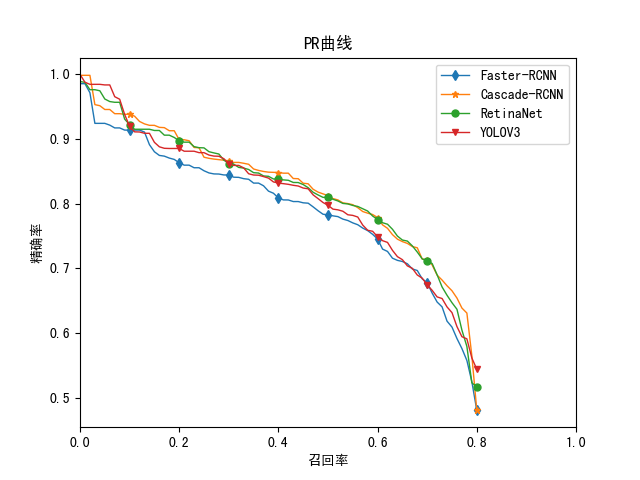
\includegraphics[width=0.6\linewidth]{PR_net.png}                      
  \caption{四种检测网络的PR曲线(IOU=0.75)}                      
  \label{fig:pr_net}       
\end{figure}   

骨髓血细胞检测是多类别检测问题,对于每一类血细胞都有自己的精确率与召回率关系。为了更加直观的比较不同网络的结果,
对于某一召回率,我们计算所有类别的平均精确率来绘制PR曲线。四种网络在$\text{IOU}=0.75$的条件下PR曲线如图~\ref{fig:pr_net}所示。
四种网络每类血细胞的PR曲线如图~\ref{fig:pr_curve}(a)-(d)所示。

\begin{figure}[htbp]
	\centering
  \begin{subfigure}{0.48\linewidth}
    \centering
    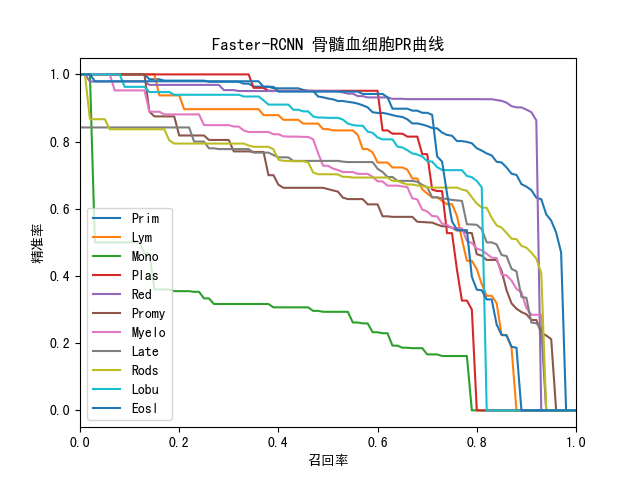
\includegraphics[width=1.0\linewidth, height=0.75\linewidth]{PR_1.png}
    \caption{Faster-RCNN网络PR曲线}
  \end{subfigure}
  \begin{subfigure}{0.48\linewidth}
    \centering
    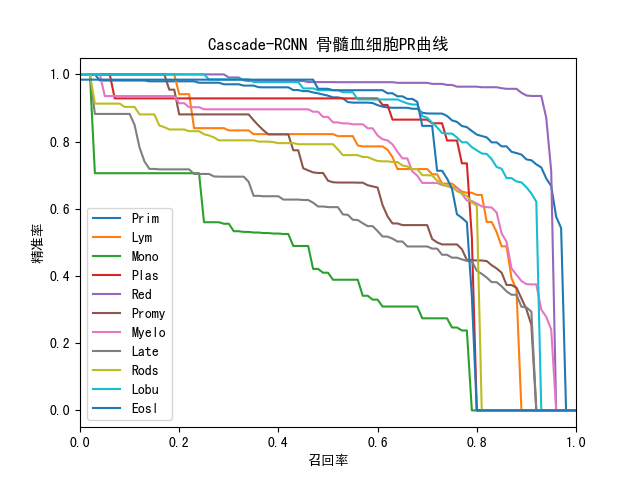
\includegraphics[width=1.0\linewidth, height=0.75\linewidth]{PR_2.png}
    \caption{Cascade-RCNN网络PR曲线}
  \end{subfigure}
	\centering
  \begin{subfigure}{0.48\linewidth}
    \centering
    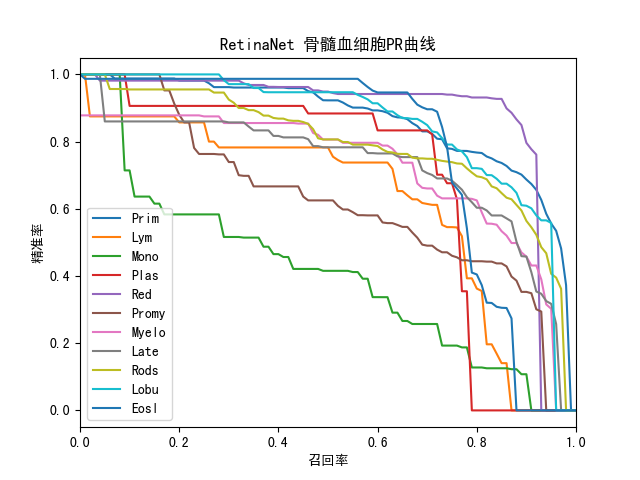
\includegraphics[width=1.0\linewidth, height=0.75\linewidth]{PR_3.png}
    \caption{RetinaNet网络PR曲线}
  \end{subfigure}
  \centering
  \begin{subfigure}{0.48\linewidth}
    \centering
    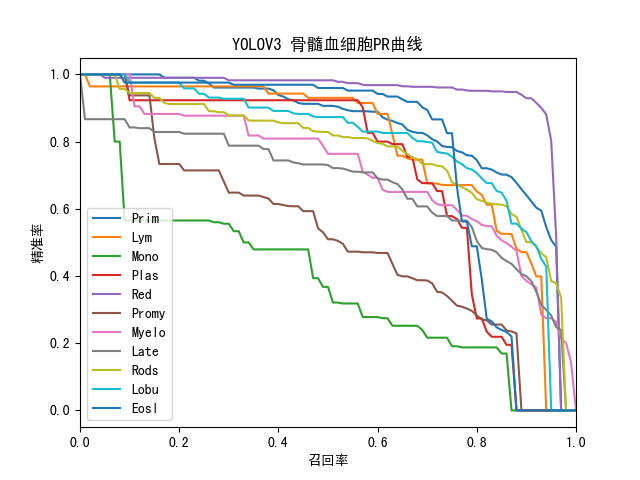
\includegraphics[width=1.0\linewidth, height=0.75\linewidth]{PR_4.png}
    \caption{YOLOV3网络PR曲线}
  \end{subfigure}
	\caption{四种检测网络的PR曲线}
	\label{fig:pr_curve}
\end{figure}

为了进一步直观了解网络的检测性能,我们将检测框进行可视化绘制,如图$~\ref{fig:detect_result}$所示,图中仅展示置信度大于0.6的检测框结果。
图中(a)为血细胞人工标注的结果,(b)-(e)为网络检测的结果。从中我们可以看出原始细胞与嗜中性中幼粒细胞易发生混淆,在第二列图像中,只有Cascade-RCNN网络检测正确,Faster-RCNN与RetianNet
均出现了虚警框。对于第四列图像中的破碎细胞,只有RetinaNet将其识别为背景,而其他网络均出现了虚警。实验结果表明,四种目标检测网络可以有效的检测并识别图像中的骨髓血细胞,
但识别的准确率有待提升。

\begin{figure}[htbp]
	\centering
	\begin{subfigure}{0.9\linewidth}
		\centering
		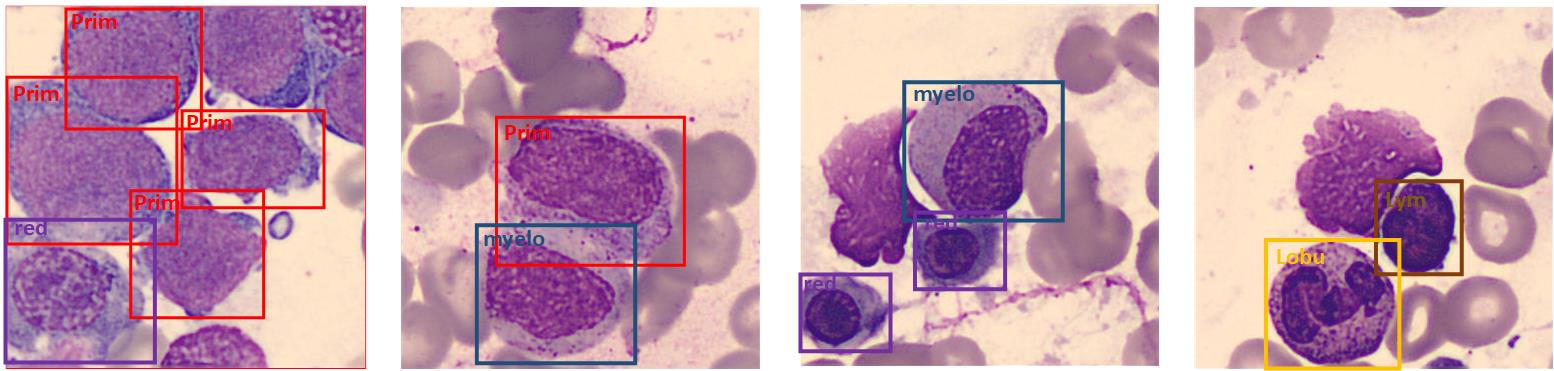
\includegraphics[width=1.0\linewidth, height=0.25\linewidth]{detect_result/gt.jpg}
    \caption{真实标注}
	\end{subfigure}
	\centering
	\begin{subfigure}{0.9\linewidth}
		\centering
		\includegraphics[width=1.0\linewidth, height=0.25\linewidth]{detect_result/faster_rcnn.jpg}
    \caption{Faster-RCNN检测结果}
	\end{subfigure}
	\centering
	\begin{subfigure}{0.9\linewidth}
		\centering
		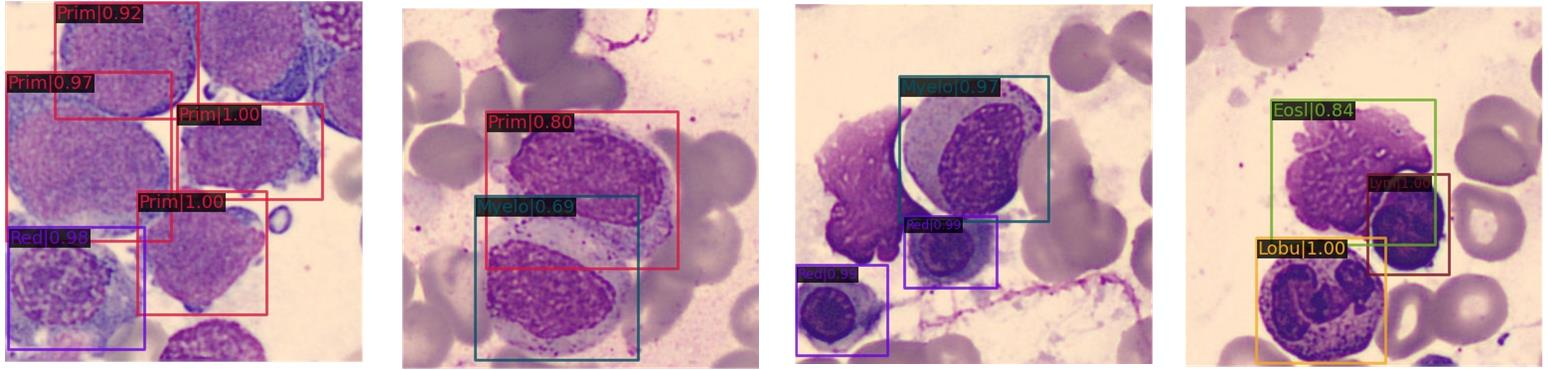
\includegraphics[width=1.0\linewidth, height=0.25\linewidth]{detect_result/cascade.jpg}
    \caption{Cascade-RCNN检测结果}
	\end{subfigure}
	\centering
	\begin{subfigure}{0.9\linewidth}
		\centering
		\includegraphics[width=1.0\linewidth, height=0.25\linewidth]{detect_result/retinanet.jpg}
    \caption{RetinaNet检测结果}
	\end{subfigure}
	\centering
  \begin{subfigure}{0.9\linewidth}
		\centering
		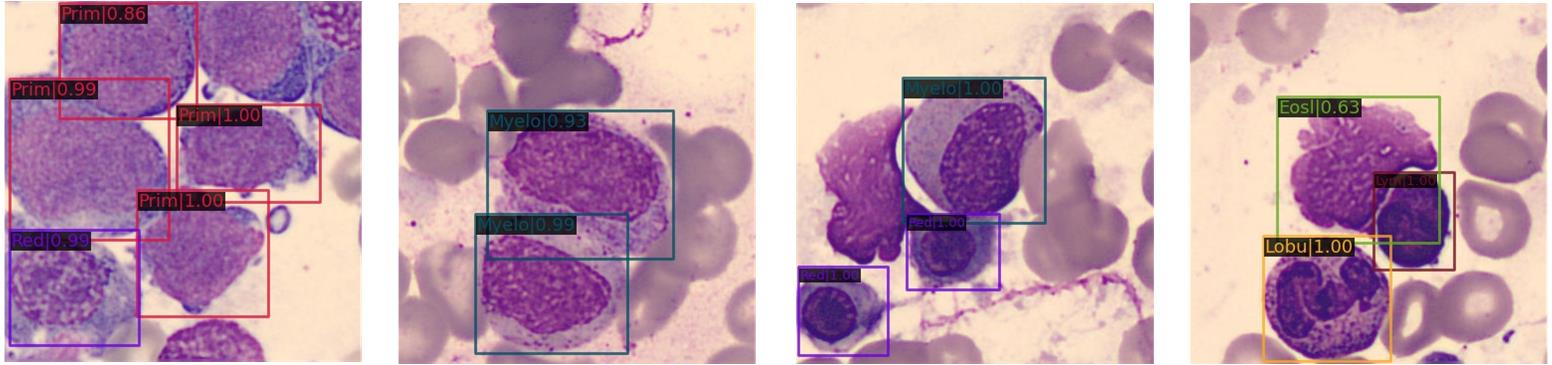
\includegraphics[width=1.0\linewidth, height=0.25\linewidth]{detect_result/YOLOV3.jpg}
    \caption{YOLOV3检测结果}
	\end{subfigure}
	\caption{四种检测网络的可视化检测结果}
	\label{fig:detect_result}
\end{figure}

综合考虑计算量,参数量与检测精度等因素,我们选择性能较为优异RetinaNet作为基线模型,并基于骨髓血细胞特性对RetinaNet进行改进。

\subsubsection{检测网络与检测识别网络性能对比}

骨髓血细胞检测识别网络需要给出骨髓血细胞的位置与类别,检测网络只需要进行前景检测输出血细胞的位置信息。
我们以RetinaNet单阶段网络作为基线模型,对比了检测网络与检测识别网络在特征图与混淆矩阵上的差异。

骨髓血细胞检测识别的混淆矩阵的定义如下,首先对网络输出的检测框
按照分类置信度进行过滤,只有分类置信度大于阈值的检测框才参与混淆矩阵的计算,然后
基于IOU与标签信息来衡量检测结果是否正确。RetinaNet检测识别网络在score(分类置信度) > 0.3、IOU=0.5条件下的混淆矩阵如图~\ref{fig:det_confusion}(a)所示。
各个类别的召回率与精确率如表~\ref{table:cell_cls}所示。单核细胞(Mono)、杆状核细胞(Rods)与嗜酸性粒细胞(Eosl)
存在比较严重的漏检的问题,召回率小于0.5。嗜中性中幼粒细胞(myelo)与嗜中性晚幼粒细胞(Late)的识准确正确率较差。
检测识别网络平均的检测正确率只有0.581。
RetinaNet检测网络在score(分类置信度) > 0.95、IOU=0.5条件下的混淆矩阵如图~\ref{fig:det_confusion}(b)所示, 骨髓血细胞的召回率0.964,正确率为0.934。
检测网络在$IOU=0.75$条件下的平均精度(AP)为0.942。实验结果表明,在仅做检测后,骨髓血细胞召回率与准确率极高,可以满足实际应用需求。

\begin{table}   
  \caption{RetinaNet网络各类别的准确率与召回率}      
  \centering    
  \label{table:cell_cls}
  \resizebox{0.8\linewidth}{!}{ 
  \begin{tabular}{ccccccc}     
    \hline    
     & prim & lym & mono &  plas & red & promy    \\ 
    \hline      
    Precision    & 0.644 & 0.621 & 0.553 & 0.783 & 0.787 & 0.512  \\      
    Recall       & 0.780 & 0.682 & 0.236 & 0.591 & 0.888 & 0.454 \\      
    \hline         
  \end{tabular} 
  }
  \centering  
  \resizebox{0.8\linewidth}{!}{ 
  \begin{tabular}{ccccccc}                 
     & myelo  & late & rods & lobu &  eosl & 平均 \\          
    \hline          
    Precision    & 0.448 & 0.439 & 0.778 & 0.715 & 0.857 &  0.581   \\      
    Recall       & 0.646 & 0.506 & 0.319 & 0.672 & 0.505 &   \\       
    \hline            
  \end{tabular} 
}  
\end{table}

\begin{figure}[htbp]                  
  \centering                   
	\begin{subfigure}{0.48\linewidth}
		\centering
    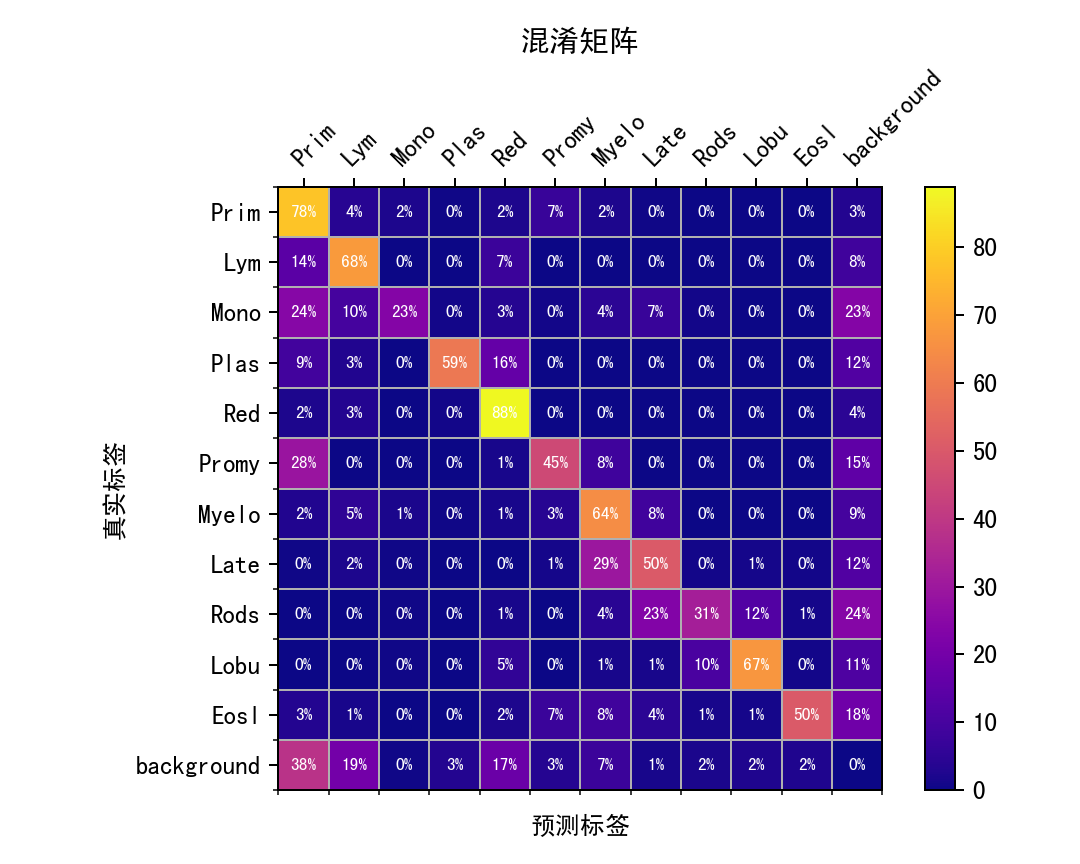
\includegraphics[width=1.0\linewidth, height=0.8\linewidth]{det_confusion.png}                   
    \caption{RetinaNet检测识别混淆矩阵}
	\end{subfigure}
	\begin{subfigure}{0.48\linewidth}
		\centering
		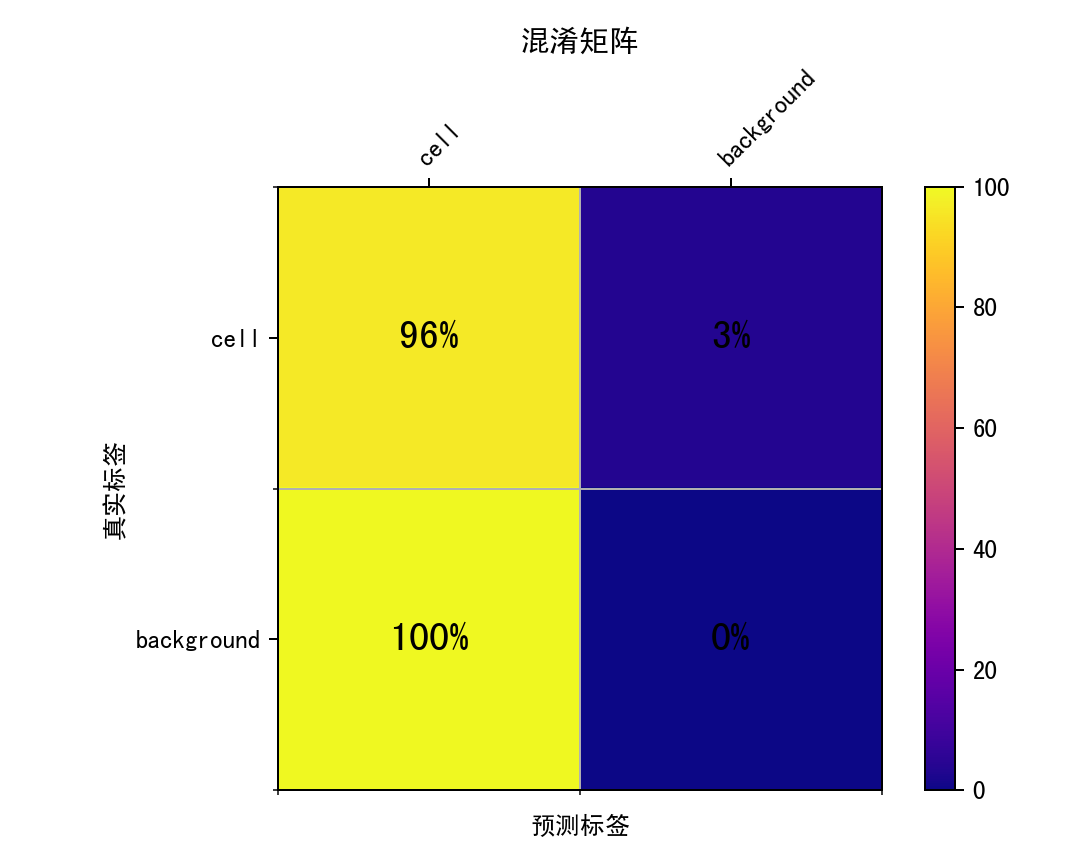
\includegraphics[width=1.0\linewidth, height=0.8\linewidth]{det_confusion1.png}
    \caption{RetianNet检测混淆矩阵}
	\end{subfigure}
  \caption{RetinaNet检测识别与检测网络的混淆矩阵}                   
  \label{fig:det_confusion}      
\end{figure}   

检测网络与检测识别网络骨干网络输出的均值特征图如图所示,第一行为检测网络骨干网络在第$2\sim 5$阶段输出的特征图,第二行为检测识别网络输出的特征图。
从图中可以发现检测网络特征图主要关注细胞的边缘信息,而检测识别网络需要关注细胞核、细胞质等全局信息。
我们认为在检测识别网络中,识别任务的难度要远高于坐标回归检测任务。识别任务需要提取精细、丰富的全局特征,
坐标回归任务只需关注中心、边缘等局部特征。两类任务虽然在头部由不同的分支进行学习,但是共享骨干网络提取的特征,
由于任务之间可能存在相互干扰,梯度更新方向不一致,导致骨干网络难以对精细分类特征进行学习,因此识别识别效果较差。

\begin{figure}[htbp]                     
  \centering                      
  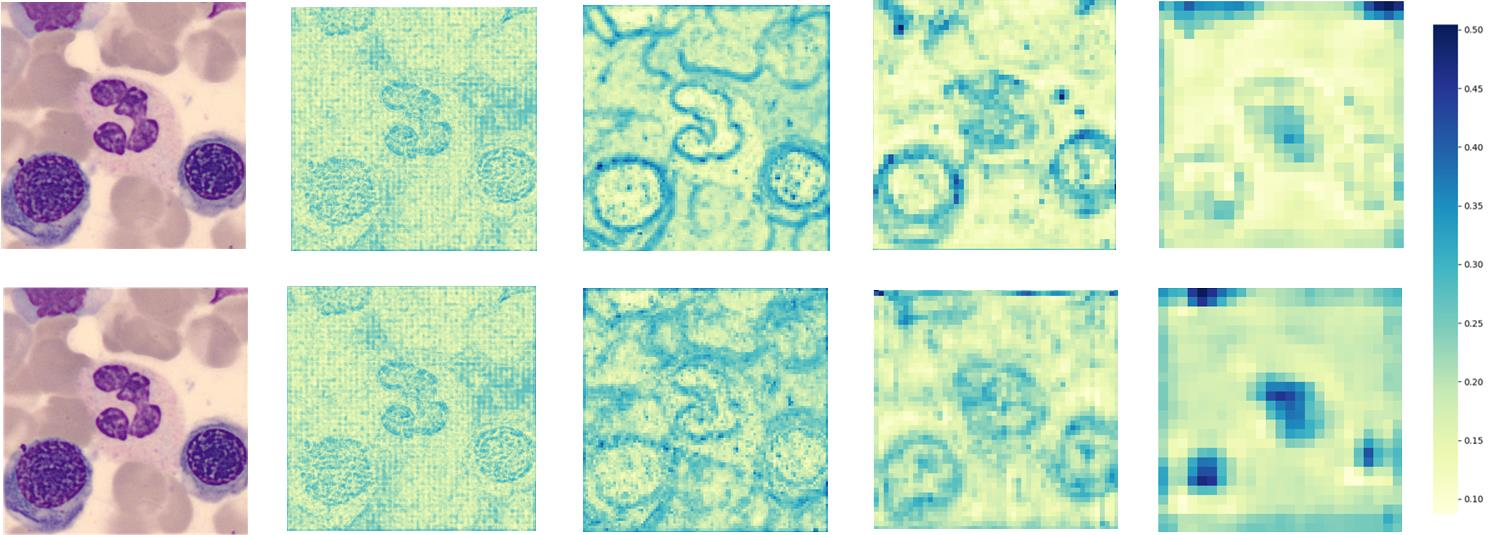
\includegraphics[width=0.95\linewidth]{features.jpg}                      
  \caption{检测网络与检测识别网络特征图对比}                      
  \label{fig:feature}       
\end{figure}   

 由于检测识别一体化的网络效果较差,不能满足实际应用的需求。因此,我们先用目标检测网络进行血细胞前景检测与坐标回归,再将血细胞裁剪为切片,
 然后使用血细胞识别网络进行识别。通过将检测任务与识别任务解耦来提高血细胞分类计数任务的准确性。

\section{小结}

针对骨髓血细胞的检测,本章首先分析对比了单双阶段目标检测网络的差异,然后评估了不同
检测网络在骨髓血细胞数据集上的检测精度、计算量与速度等性能。实验结果表明RetinaNet单阶段网络
在速度与精度上要优于其他检目标检测网络,因此我们选择将其作为骨髓血细胞检测的基线模型。此外我们对比了检测网络与
检测识别网络在特征提取与识别准确率上的差异, 实验结果表明检测识别网络的输出类别置信度较低,平均识别正确率只有58.1\%,
易发生漏检与误检。检测网络的平均精度达到了94.2\%,网络检测的准确率与召回率都有大幅提升。
因此我们确定了先检测再识别的骨髓血细胞处理流程,即先使用检测网络定位到血细胞的位置,然后剪切为血细胞切片,
再输入到识别网络中进行分类。



